%Capítulo 2

\section{Antecedentes}
    
    En esta sección  se describen diversos proyectos, artículos científicos, así como proyectos de tesis que tengan relación con el desarrollo de la red \Gls{LoRaWAN} o en otras tecnologías similares.

\subsection{Puerta de acceso IoT con Computación de frontera para la Monitorización Agrícola} 

  Este artículo científico \cite{iot_gateway} habla sobre el diseño de una puerta de acceso basado en \gls{Computacion de frontera} para el monitoreo del crecimiento de cultivos. Para esto se utiliza tecnología de contenedores virtualizados para empaquetar todas las herramientas necesarias para el uso del protocolo \Gls{LoRaWAN}  en un servidor, herramientas de identificación de pestes e información del entorno a través de funciones que conviertan datos en imágenes.
  El puente de acceso aplica una capa intermedia de software orientada al uso de mensajes para estandarizar y personalizar la transmisión de datos entre funciones, nubes y fronteras. A través de la simulación y datos de campo el diseño de la puerta de acceso puede obtener las funciones y datos de cada módulo al mismo tiempo, así como la utilización y transmisión con una gran calidad y estabilidad. 
  A continuación en la Figura \ref{arquitecturacloudedgesensors} una imagen demostrando la relación entre la nube, \gls{Computacion de frontera} y las terminales:
  \begin{figure}[H]
  \centering
  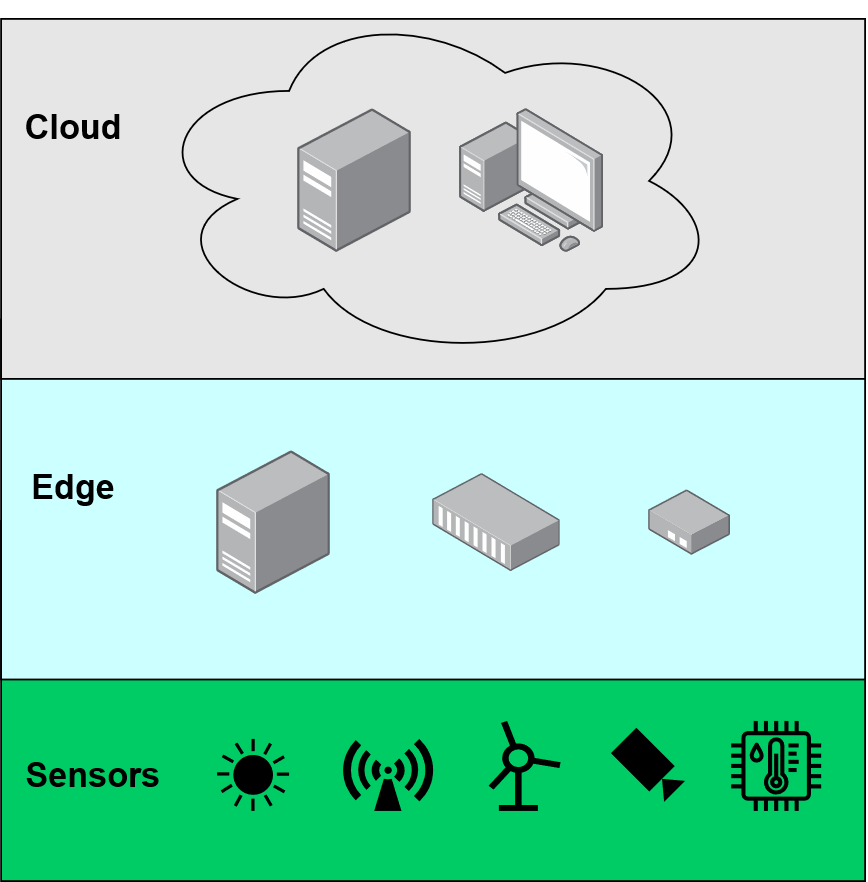
\includegraphics[width=0.8\textwidth]{imagenes/ArquitecturaCloudEdgeSensors.PNG}
  \caption{Relación entre la nube, computación de frontera y terminales}
  \label{arquitecturacloudedgesensors}
  \end{figure}
  
  A si mismo, en la Figura \ref{edgecomputinggateway} se muestra una imagen con la arquitectura de la puerta de enlace:
  
  \begin{figure}[H]
  \centering
  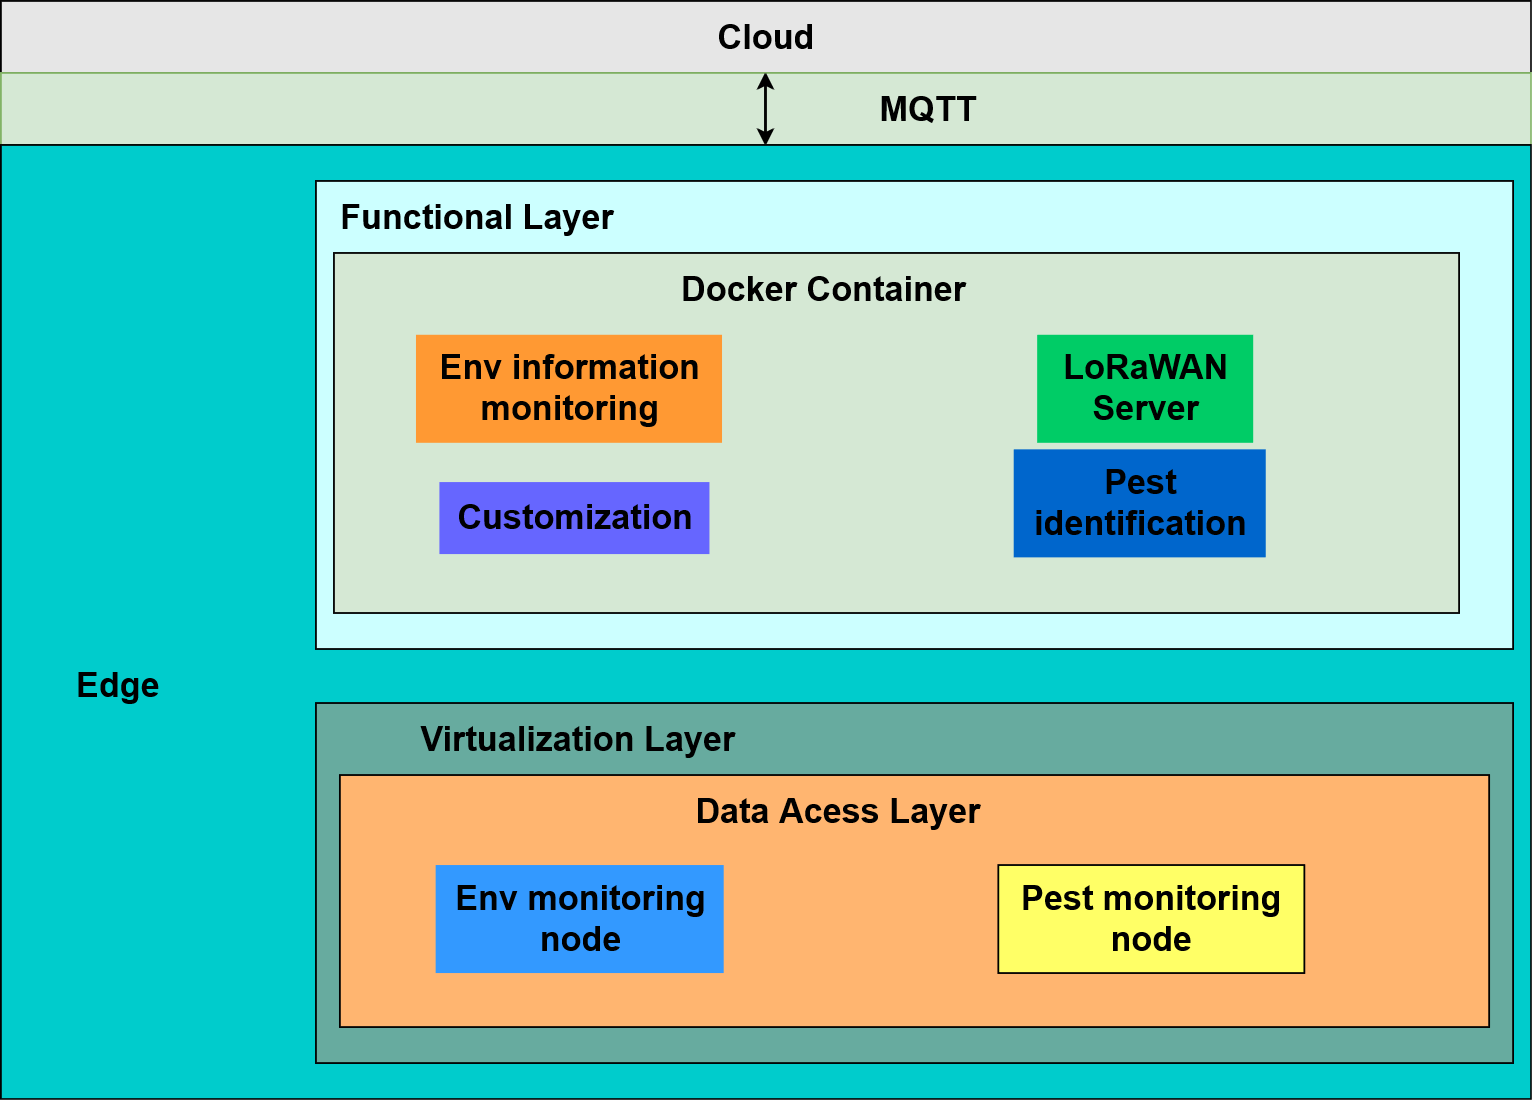
\includegraphics[width=0.8\textwidth]{imagenes/EdgeComputingGateway.PNG}
  \caption{Arquitectura de la puerta de enlace o computación de frontera}
  \label{edgecomputinggateway}
  \end{figure}
  
  \newpage

Los resultados de la investigación demostraron que \gls{Computacion de frontera} tiene la ventaja de ser de bajo costo, baja latencia y bajo consumo de poder lo que la vuelve con gran potencial para uso práctico. Así mismo el apoyo de tecnologías de contenerización y la computación en la nube vuelven al proyecto mas robusto frente a errores y la búsqueda de replicación o escalación de estas funcionalidades y se reportan terminos de reportan una tasa media de éxito en la transmisión de datos del 99,1 por ciento, con el objetivo de reducir la latencia y la carga de los servidores en la nube. 

\subsection{Evaluación experimental de sensores en un sistema de seguimiento GPS basado en LoRaWAN}

El siguiente artículo \cite{tracking_system_lora} científico se enfoca en proveer una solución basada en LoRaWAN para el desarrollo de ciudades inteligentes con el uso de sensores en
 un sistema de seguimiento GPS basado en LoRaWAN, una tecnología de comunicación inalámbrica de bajo consumo y largo alcance. 
Su objetivo es analizar el funcionamiento de los sensores y el rendimiento del sistema para la localización y transmisión de datos, 
considerando las características de esta tecnología en aplicaciones de seguimiento remoto e IoT.
El artículo resalta los beneficios de esta tecnología como es su bajo costo y poder de consumo comparado con distintas alternativas. 
A través de esta investigación el equipo de desarrollo implementa un sistema de rastreo de una flota de vehículos utilizando LoRaWAN usando como caso de estudio la ciudad de Kozani en Grecia.
La arquitectura es utilizada de la siguiente forma en la Figura \ref{applicationarchitecture}. 
Como se puede ver esta es ligeramente distinta al artículo anterior, pero cabe destacar que es bastante estándar dentro de los modelos LoRa como veremos mas adelante en el marco teórico. 

  \begin{figure}[H]
  \centering
  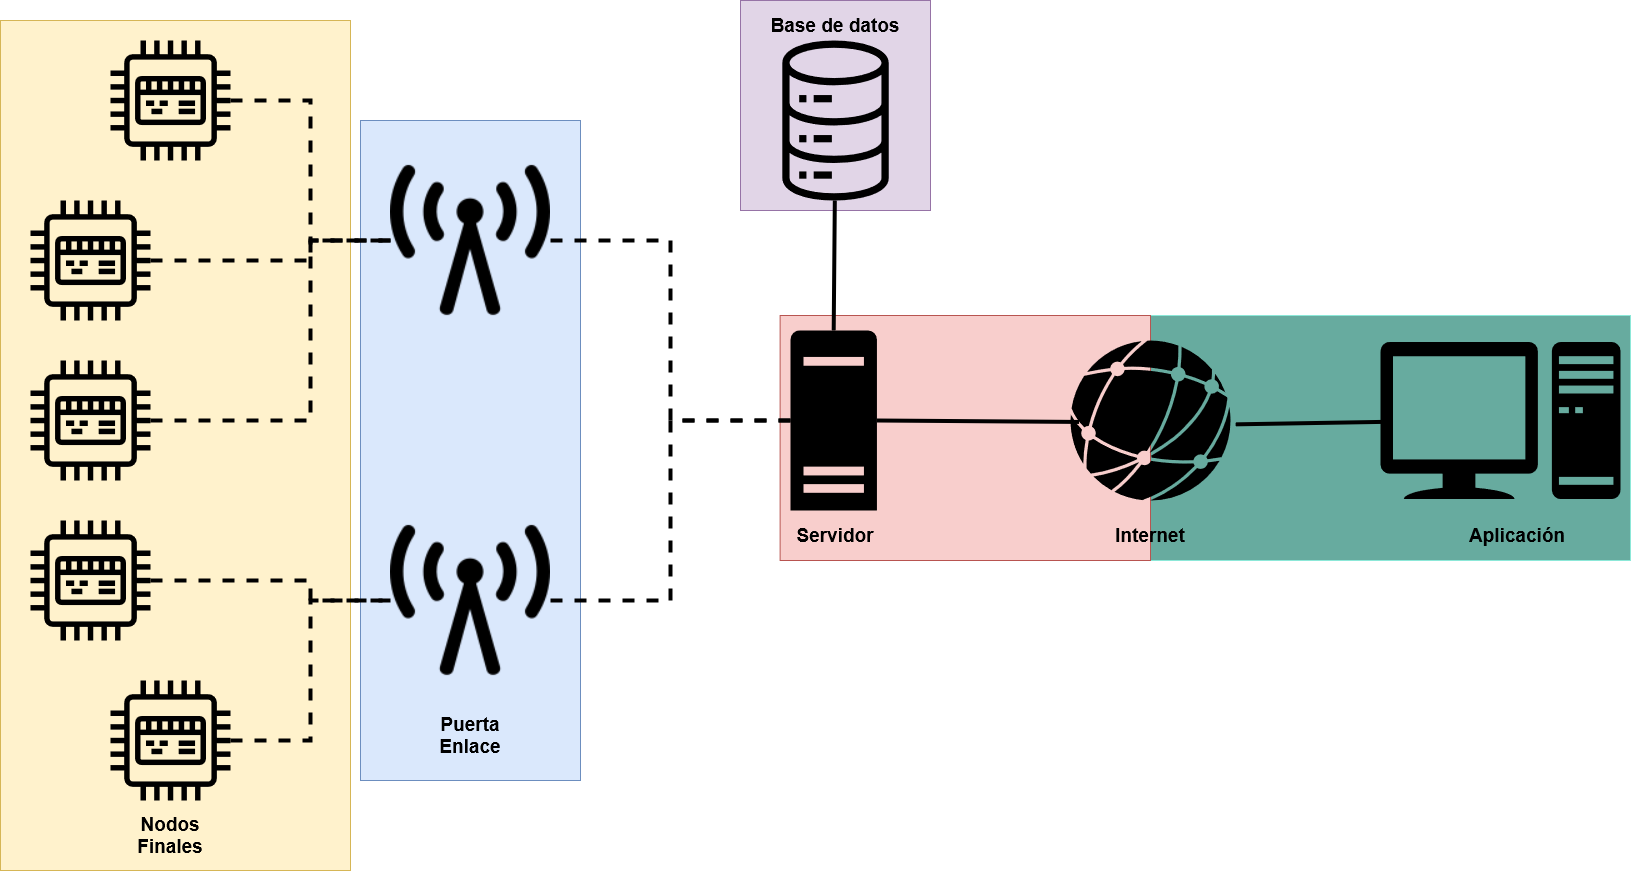
\includegraphics[width=1.1\textwidth]{imagenes/LoRaWAN-Arch.PNG}
  \caption{Arquitectura de la aplicación}
  \label{applicationarchitecture}
  \end{figure}

De izquierda a derecha la arquitectura muestra un sistema de nodos finales basados en antenas GPS comunicándose con puertas de enlace a través de LoRaWAN, estos últimos a su vez redirigen los datos a un servidor donde guardan la información en una base de datos y a través de internet llegan a una aplicación utilizando The Things Network de la cual se hablará mas adelante en el marco teórico.

\subsection{Implementación de LoRaWAN desde el dispositivo final hasta la aplicación}

Este artículo \cite{lorawan_app} habla sobre la implementación de una red completa LoRaWAN. El sistema resultante ofrece una infraestructura completa para el desarrollo de aplicaciones y
 experimentos. La red consiste en tres componentes principales. La herramienta llamada Chirpstack que es de código libre y actúa como un servidor LoRaWAN corriendo en una 
 computadora personal. La puerta de enlace LoRaWAN que es un dispositivo de red independiente y la referencia al dispositivo final que está 
 construida con componentes baratos para los autores. 

El proyecto cuenta con distintos esquemáticos ligados a través de referencias bibliográficas del dispositivo o nodo final para su fácil replicación. 
Así mismo la jerarquía utilizada para comunicar todos los dispositivos es la siguiente demostrada en la Figura \ref{fig:JerarquiaLoRaWAN} 

\begin{figure}[H]
    \centering
    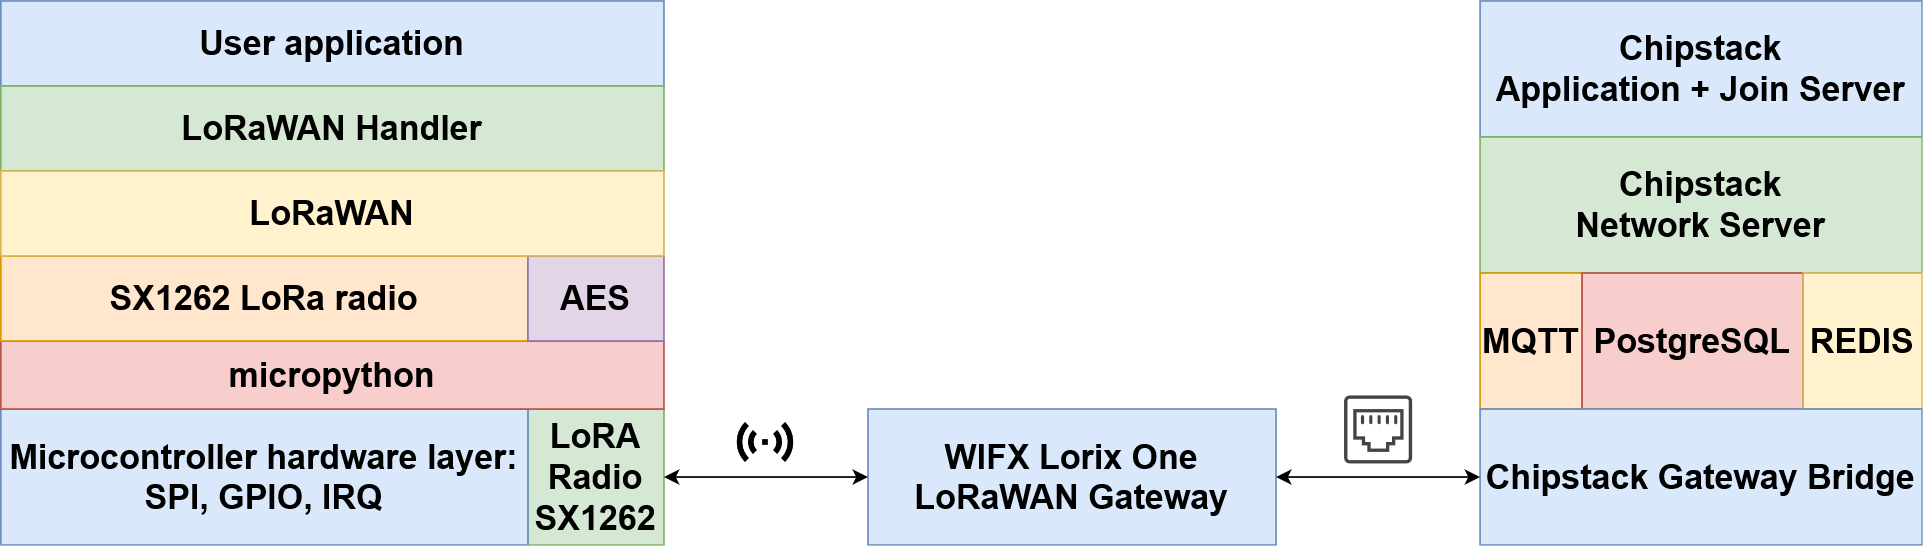
\includegraphics[width=1.0\textwidth]{imagenes/JerarquiaLoRaWAN.png}
    \caption{Jerarquía de componentes LoRa}
    \label{fig:JerarquiaLoRaWAN}
\end{figure}

Así mismo la solución propuesta por los autores esta implementada en MicroPython y se aprovecha de librerías existentes para el manejo de la tecnología y comunicación LoRaWAN.  

El servidor de red LoRaWAN está corriendo en una computadora personal aprovechando las capacidades de Docker para la generación de toda la capa de herramientas necesarias para su funcionamiento. 

Como resultados, los autores lograron obtener un servidor totalmente funcional corriendo en un contenedor que a su vez registra eventos ocurridos en el dispositivo final. 
Se hablan de las características pendientes por implementes, sin embargo, están satisfechos con el resultado debido a que la red es completamente funcional sin estas características. 

\subsection{Adquisición flexible de datos mediante LoRaWAN y MQTT para pequeñas y medianas empresas}

 Este artículo \cite{lorawan_mqtt_data_acquisition} propone una solución de LoRaWAN y MQTT para pequeñas y medianas empresas, presentando una solución generalizada para distintos tipos 
 de problemas que evade altos costos de inversión y poder obtener datos en un periodo corto de tiempo además la solución está basada en herramientas de código abierto, 
 obteniendo las ventajas de este tipo de herramientas. 
 
El enfoque propuesto es el siguiente en la Figura \ref{arquitecturaLoraGeneralPropuesta}

\begin{center}
    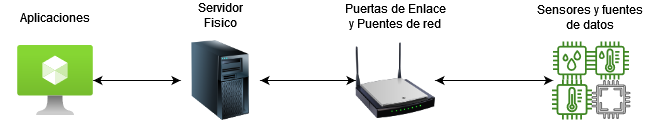
\includegraphics[width=1.0\textwidth]{imagenes/LoraWanAppProp.png}
    \captionof{figure}{Arquitectura general propuesta}
    \label{arquitecturaLoraGeneralPropuesta}
\end{center}

El artículo contribuye en proponer una solución flexible y con una infraestructura simple para la adquisición de datos a través de una red de sensores LoRaWAN y su visualización a través de una plataforma de Internet de las Cosas.

El protocolo MQTT funciona como intermediario entre LoRaWAN y la arquitectura del servidor asi como habilitador para la transferencia de datos de otras fuentes.

Asi mismo, este contribuye en aplicaciones practicas y actuales usando sensores de LoRaWAN asi como maneras de comunicarse a través de MQTT.

La solución propuesta viene de 3 componentes principales como se muestra en la Figura \ref{arquitecturaLoraGeneralPropuesta_2}:
\begin{itemize}
    \item Centro de datos
    \item Adquisición de datos con LoRaWAN
    \item Plataforma de Internet de las cosas
\end{itemize}

\begin{center}
    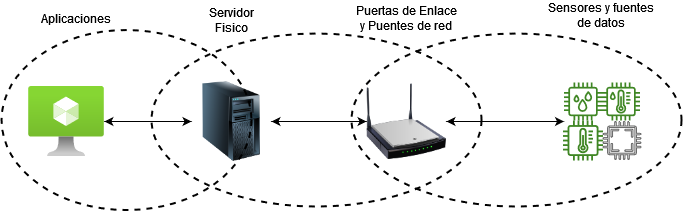
\includegraphics[width=1.0\textwidth]{imagenes/LoraWanComponentes.png}
    \captionof{figure}{Arquitectura general propuesta}
    \label{arquitecturaLoraGeneralPropuesta_2}
\end{center}


El protocolo intermediario MQTT es el centro de datos, diseñado para la conexión con dispositivos de recursos limitados. También este mismo habilita la comunicación entre 
sistemas utilizando el patrón de diseño de publicación y suscripción como se muestra en la Figura \ref{arquitecturaMQTTPropuesta}.

\begin{center}
    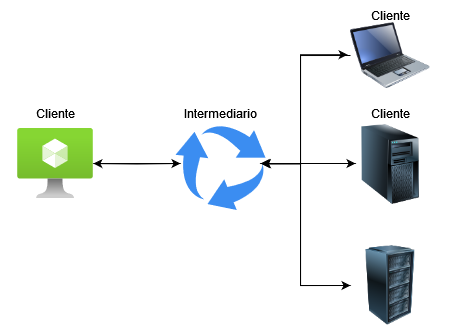
\includegraphics[width=1.0\textwidth]{imagenes/MQTTConcept.png}
    \captionof{figure}{Arquitectura MQTT propuesta}
    \label{arquitecturaMQTTPropuesta}
\end{center}


El protocolo LoRaWAN es utilizado como una red inalámbrica de sensores, proporcionando una comunicación de larga distancia.
Los sensores operados por batería son fácilmente desplegables en este tipo de protocolos y son integrados a través de una interfaz web, 
lo que hace que no sea necesario conocimientos de programación para su administración como se puede ver en la Figura \ref{arquitecturaLoRaWANPropuesta}.

\begin{center}
    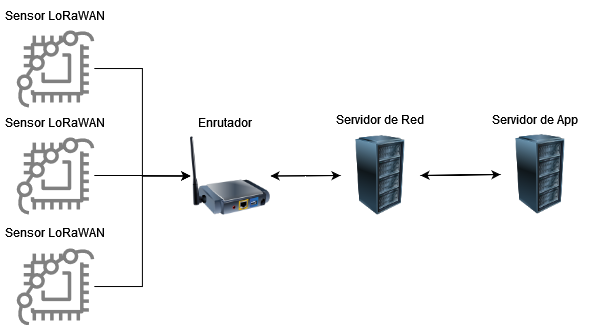
\includegraphics[width=1.0\textwidth]{imagenes/LoRaWANConcept.png}
    \captionof{figure}{Arquitectura LoRa propuesta}
    \label{arquitecturaLoRaWANPropuesta}
\end{center}


La plataforma IoT es desplegada como se ve en la Figura \ref{arquitecturaIoTPropuesta} y utilizada para medir los datos obtenidos en un panel web. Esto propicia a una visualización y medición con poco esfuerzo, 
además de permitir agregar otras fuentes de datos gracias a su integración con MQTT

\begin{center}
    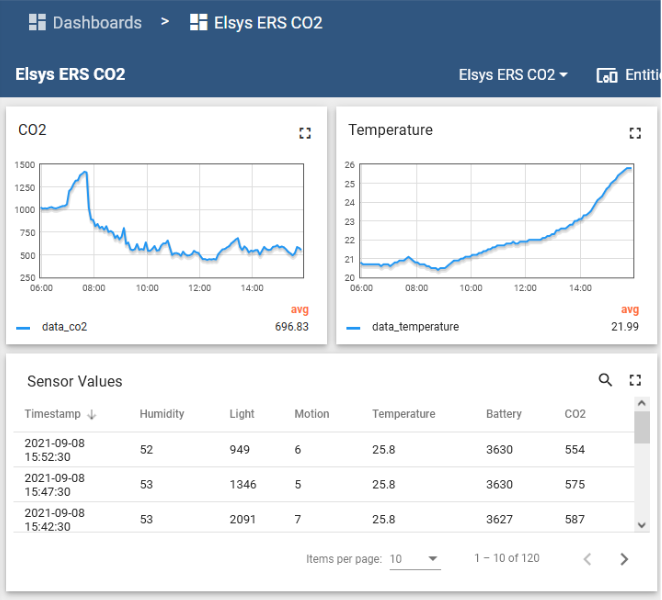
\includegraphics[width=1.0\textwidth]{imagenes/PlataformaIoT.png}
    \captionof{figure}{Plataforma IoT propuesta}
    \label{arquitecturaIoTPropuesta}
\end{center}

El sistema implementado puede gestionar aproximadamente 5.000 mensajes MQTT por segundo con cargas útiles inferiores a 1.000 bytes, según la evaluación de rendimiento 
presentada por los autores.
En conclusión, este trabajo demuestra el conjunto de herramientas en un solo proyecto con múltiples tipos de aplicación, el cual definitivamente es una buena base para 
el presente proyecto.

\subsection{Diseño de una pasarela LoRaWAN con servidores autónomos para comunidades sin conexión a Internet}

Este artículo \cite{local_things_network} habla de como los dispositivos IoT en la práctica deberían ser sencillos de desplegar asi como deberían durar activos 
largos periodos en campo sin ninguna intervención. Se propone el uso del protocolo LoRaWAN para conseguir estos objetivos, además, se habla del uso de un conjunto de 
herramientas llamado The Things Networks el cual en Europa es fácilmente accesible ya que cuenta con dispositivos usables en campo para conectar con dispositivos LoRaWAN finales.

Debido a que no se puede garantizar siempre tener internet en muchos países, se propone una solución utilizando nodos IoT locales a una puerta de enlace LoRaWAN sin la 
necesidad de emplear redes de internet, a un bajo costo y poco poder de consumo. 

Los investigadores implementaron tres bloques de la arquitectura LoRaWAN (Puerta de enlace, Servidor de Red, Servidor de Aplicación) en un solo dispositivo utilizando una Raspberry Pi 
y un modulo LoRaWAN. 
El acceso local a los datos de la aplicación es a través de un punto de acceso WiFi, permitiendo a los miembros de la comunidad acceder a sus datos comunitarios incluso cuando no hay 
internet. Además de datos IoT en tiempo real, los investigadores proponen servicios extra que pueden ser implementados en el repositorio para ayudar en el desarrollo de la educación, 
salud y otros contenidos que pueden apoyar a comunidades distantes. 

\begin{center}
    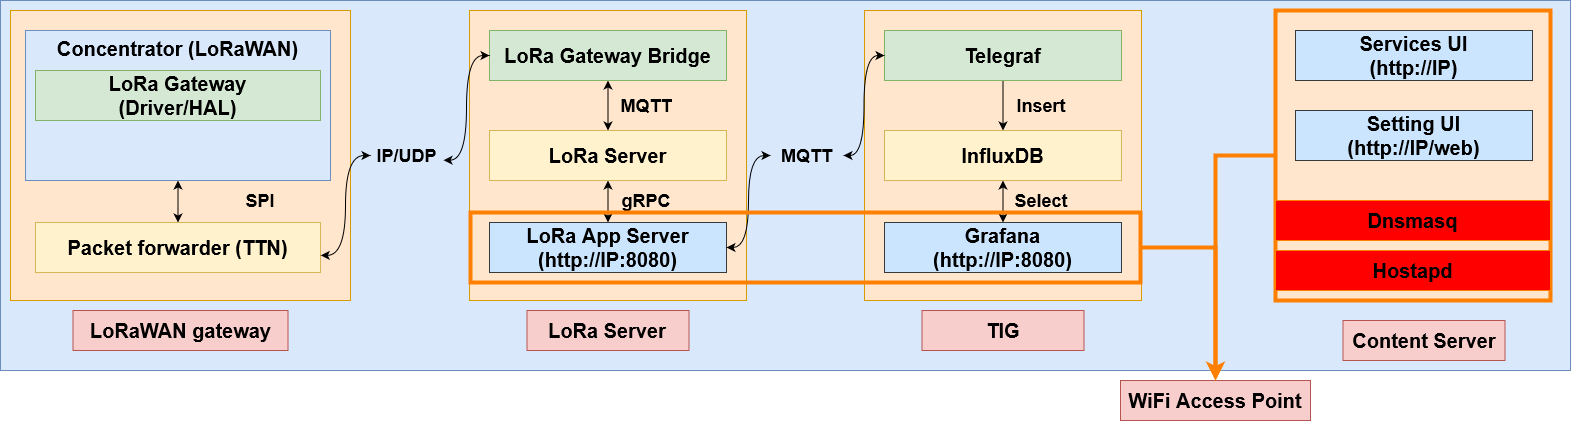
\includegraphics[width=1.0\textwidth]{imagenes/PartsOfBS.png}
    \captionof{figure}{Partes de una Estación Base}
    \label{PartsOfBaseStation}
\end{center}

El dispositivo completo con todas estas características es llamado la Estación Base (BS en inglés).
La arquitectura de la estación base es dividida en cuatro partes como se muestra en la Figura \ref{PartsOfBaseStation}: Puerta de enlace LoRaWAN (GW en inglés), Servidor de aplicación y de red, un componente llamado TIG (De las siglas Telegraf, InfluxDB y Grafana), el punto de acceso WiFi y el servidor de contenido

Puerta de Enlace LoRaWAN Figure \ref{BSwith8and1channel}. Actúa como un transmisor de paquetes entre un nodo final y un servidor de red basado en la implementación de código abierto propuesta por Semtech y 
construida en una Raspberry Pi. El equipo de investigadores cuenta con dos versiones, la más robusta que usa un módulo SX1301 la cual admite comunicación simultanea mientras escucha en ocho diferentes frecuencias y la mas barata utilizando un módulo RFM96W el cual solo admite un solo canal.

Servidor de red y servidor de aplicación. El rol del servidor de red es autenticar nodos y estar seguro de que solo se reciben datos de los dispositivos registrados. 
El servidor de aplicación provee procesamiento de tramas y su desencriptación. Asi mismo, ofrece al usuario final los datos solicitados, como el clima, la calidad del aire, alarmas, etc.
 Los datos son localmente procesados, guardados y se pueden accesar a través del punto de entrada WiFi 

TIG. La herramienta de Telegraf es usada para suscribirse a un intermediario de mensajes MQTT y recolectar mensajes en formato JSON los cuales son transmitidos por el servidor de
 aplicación LoRa y esto se inyectan en InfluxDB una base de datos de series de tiempo (TSDB en inglés). Gracias a Grafana (Una plataforma de código abierto para gráfico de datos) las mediciones pueden ser obtenidas de InfluxDB para su análisis y monitoreo.

Servidor de Contenido. El servidor de contenido provee acceso al contenido estático, como el material educacional, información de salud, las mejores prácticas de agricultura, etc. 
Asi como un tablero que funciona como boletín de información para la comunidad. El punto de acceso WiFi hace este material disponible a través de la comunidad usando una interfaz web. 

\begin{center}
    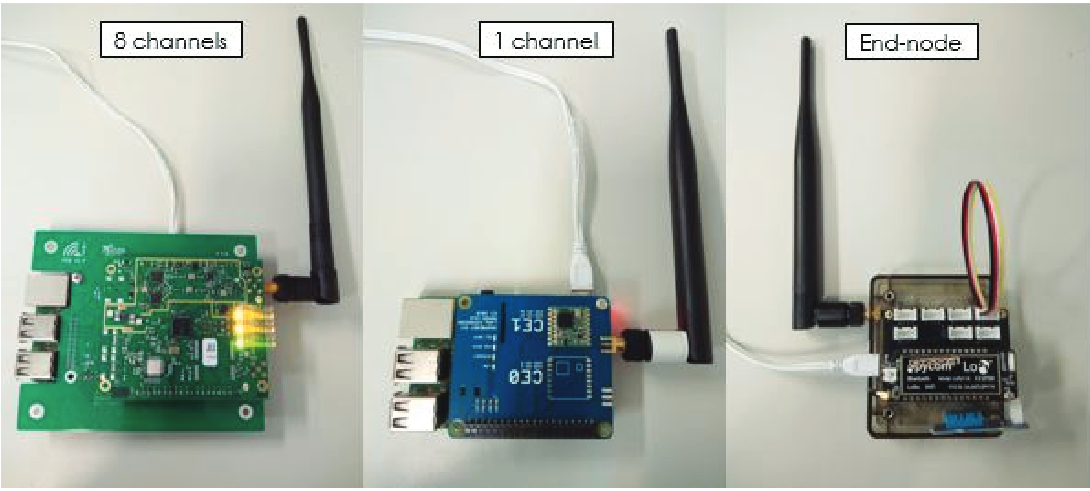
\includegraphics[width=1.0\textwidth]{imagenes/NodosPaper3.png}
    \captionof{figure}{BS con 8 canales (izquierda), 1 canal (centro) y un nodo final (derecha).}
    \label{BSwith8and1channel}
\end{center}

En conclusión, este trabajo está enfocado a extender los beneficios de utilizar IoT en personas que viven en áreas con muy limitado o sin acceso a conexiones de internet, utilizando redes y servidores LoRaWAN los cuales pueden ser encapsulados en dispositivos pequeños que proveen todas las funcionalidades requeridas. Asi mismo pueden tomar ventaja de dispositivos TTN si es que están disponibles, de forma intermitente, incluso pueden ser soluciones independientes que sirvan a una comunidad. Los usuarios pueden interactuar con el BS propuesto utilizando sus dispositivos propios a través de la conexión WiFi.
El trabajo futuro de los investigadores se centrará en el tablón de anuncios y el contenido sistemas de gestión que son características muy útiles para comunidades aisladas, así como en una extensión de este modelo al acomodar la sincronización de la base de datos de varias BS desplegadas en la misma comunidad, interconectadas entre sí pero independientes de una conexión a Internet.

\subsection{Particionado de red de acceso radio en redes LoRaWAN}

En el siguiente trabajo de final de grado \cite{particionado_de_red_lorawan} vemos que en este se propone dividir los recursos de una red LoRaWAN en segmentos o 
\textit{slices}, que puedan asignarse a distintos usuarios o proveedores. Para ello, define un bloque de recursos (RB) como la combinación de un canal y un 
factor de dispersión (SF). En la configuración estudiada, los ocho canales de 125 kHz y los SF del 7 al 12 permiten formar hasta 48 combinaciones de recursos.

La solución se implementa sobre una red LoRaWAN con ChirpStack y dispositivos reales. El servidor asocia cada dispositivo con un \textit{slice} y, durante el 
intercambio de mensajes de unión, envía al dispositivo una máscara que indica los RB disponibles. A partir de esa máscara, el dispositivo selecciona un RB y 
configura el canal y el SF de transmisión según las condiciones de la señal, estimadas mediante el indicador de fuerza de señal recibida (RSSI) o la relación 
señal-ruido (SNR). Así, la selección del SF puede ajustarse a la calidad del enlace, mientras que la separación por canal y SF permite organizar las transmisiones 
de distintos usuarios.

La arquitectura utilizada para implementar esta solución se resume en la Figura \ref{arquitecturaParticionadoLoRaWAN}. Las micro tarjetas o como el autor se refiere 
motas de modelo LoPy4 se comunican con la pasarela mediante LoRaWAN, y esta reenvía los paquetes al servidor, donde ChirpStack y el sistema de 
particionado gestionan la asignación de recursos.

\begin{center}
    \begingroup
    \shorthandoff{<>}
    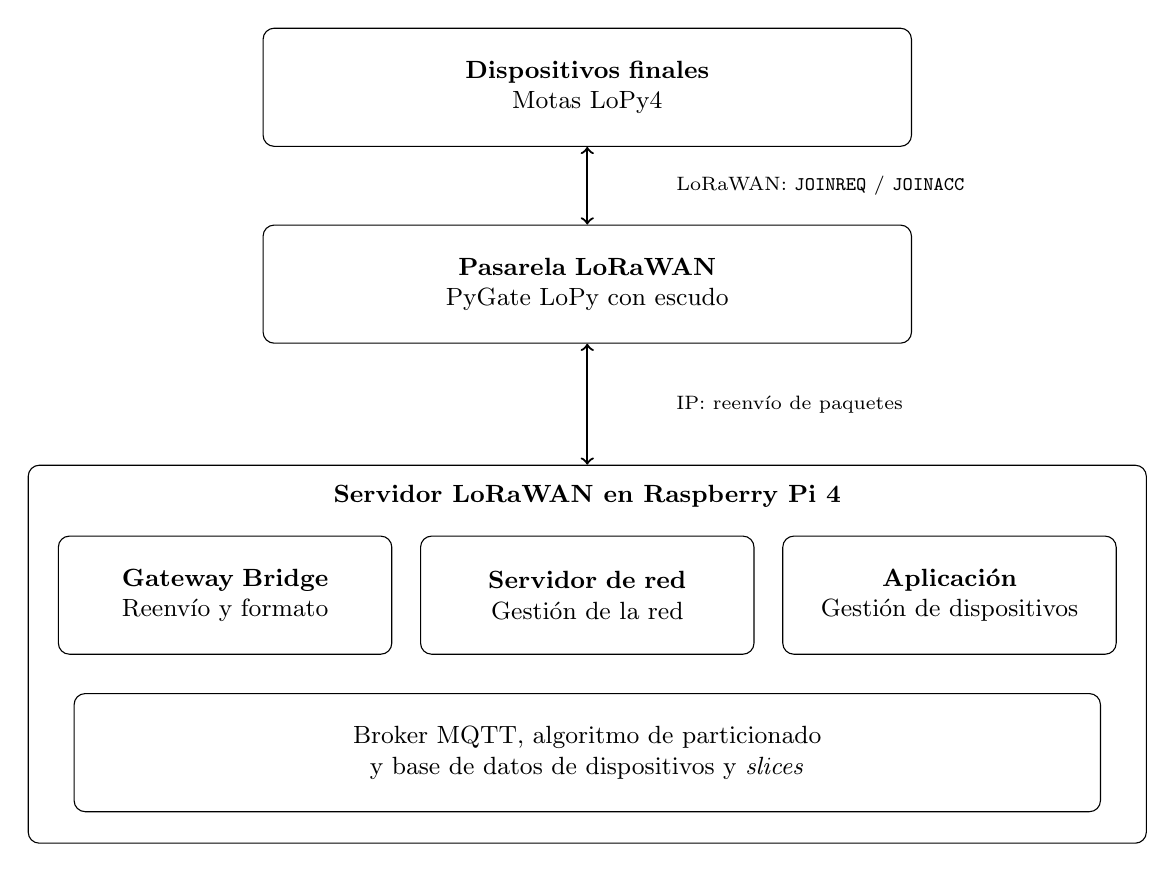
\begin{tikzpicture}[font=\small]
        \node[draw, rounded corners, align=center, text width=8cm, minimum height=1.5cm]
            (motas) at (0,0) {\textbf{Dispositivos finales}\\Motas LoPy4};

        \node[draw, rounded corners, align=center, text width=8cm, minimum height=1.5cm]
            (gateway) at (0,-2.5) {\textbf{Pasarela LoRaWAN}\\PyGate LoPy con escudo};

        \draw[<->, thick] (motas.south) -- node[midway, xshift=1cm, anchor=west, align=left]
            {\scriptsize LoRaWAN: \texttt{JOINREQ} / \texttt{JOINACC}} (gateway.north);

        \node[draw, rounded corners, minimum width=14.2cm, minimum height=4.8cm]
            (servidor) at (0,-7.2) {};
        \node[align=center] at (0,-5.2)
            {\textbf{Servidor LoRaWAN en Raspberry Pi 4}};

        \node[draw, rounded corners, align=center, text width=4cm, minimum height=1.5cm]
            at (-4.6,-6.45) {\textbf{Gateway Bridge}\\Reenvío y formato};
        \node[draw, rounded corners, align=center, text width=4cm, minimum height=1.5cm]
            at (0,-6.45) {\textbf{Servidor de red}\\Gestión de la red};
        \node[draw, rounded corners, align=center, text width=4cm, minimum height=1.5cm]
            at (4.6,-6.45) {\textbf{Aplicación}\\Gestión de dispositivos};
        \node[draw, rounded corners, align=center, text width=12.8cm, minimum height=1.5cm]
            at (0,-8.45) {Broker MQTT, algoritmo de particionado\\y base de datos de dispositivos y \textit{slices}};

        \draw[<->, thick] (gateway.south) -- node[midway, xshift=1cm, anchor=west, align=left]
            {\scriptsize IP: reenvío de paquetes} (servidor.north);
    \end{tikzpicture}%
    \endgroup
    \captionof{figure}{Arquitectura utilizada para el particionado de la red LoRaWAN}
    \label{arquitecturaParticionadoLoRaWAN}
\end{center}

Las pruebas confirmaron la comunicación entre los dispositivos y el servidor, así como la asignación de recursos según el SNR. En particular, las simulaciones 
mostraron que, para los valores de SNR evaluados, el algoritmo no asignaba factores de dispersión incompatibles con la calidad de la señal. En cambio, no fue posible 
validar el algoritmo basado en RSSI, pues durante las pruebas no se alcanzaron condiciones de cobertura suficientes para que funcionara. El trabajo concluye que el 
particionado propuesto es viable en LoRaWAN y plantea como líneas futuras ampliar los criterios de selección, analizar el rendimiento y el consumo energético, y permitir 
que el usuario elija el \textit{slice} según los requisitos de calidad de servicio.

\subsection{Diseño de un Nodo LoRa-GPS para Localización de Bicicletas Implementado en una Red LoRaWAN}

El trabajo de fin de grado de Jairo Andrés Rodríguez Sánchez y Jhoiner Smith Rojas González \cite{nodo_lora_gps} aborda el diseño de un nodo para 
localizar bicicletas mediante la integración de posicionamiento GPS y comunicación LoRaWAN. A nivel funcional, el nodo obtiene las coordenadas de la 
bicicleta y las transmite a través de la red para que puedan ser recibidas y consultadas por el usuario. Este enfoque aprovecha el alcance de LoRaWAN 
para comunicar un dispositivo móvil con una aplicación de seguimiento.

La Figura \ref{arquitecturaNodoLoRaGPS} presenta un esquema general del flujo de información: desde la obtención de la posición en la bicicleta hasta 
su consulta en la aplicación. Se muestran los componentes funcionales de una arquitectura LoRaWAN, sin especificar modelos de hardware ni plataformas 
de software particulares.

\begin{center}
    \begingroup
    \shorthandoff{<>}
    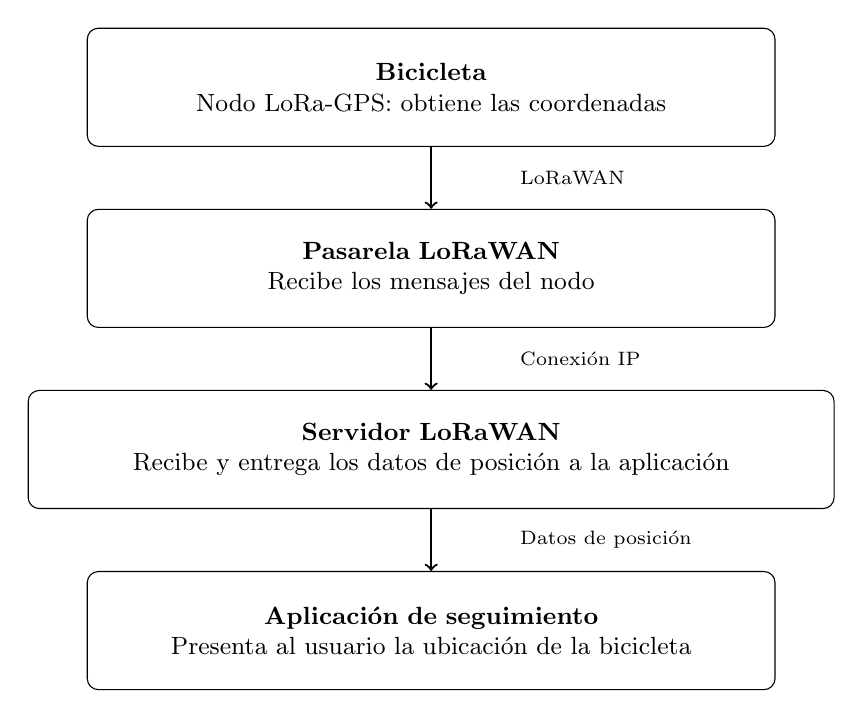
\begin{tikzpicture}[font=\small]
        \node[draw, rounded corners, align=center, text width=8.5cm, minimum height=1.5cm]
            (bicicleta) at (0,0)
            {\textbf{Bicicleta}\\Nodo LoRa-GPS: obtiene las coordenadas};

        \node[draw, rounded corners, align=center, text width=8.5cm, minimum height=1.5cm]
            (gateway) at (0,-2.3)
            {\textbf{Pasarela LoRaWAN}\\Recibe los mensajes del nodo};

        \draw[->, thick] (bicicleta.south) -- node[midway, xshift=1cm, anchor=west]
            {\scriptsize LoRaWAN} (gateway.north);

        \node[draw, rounded corners, align=center, text width=10cm, minimum height=1.5cm]
            (servidor) at (0,-4.6)
            {\textbf{Servidor LoRaWAN}\\Recibe y entrega los datos de posición a la aplicación};

        \draw[->, thick] (gateway.south) -- node[midway, xshift=1cm, anchor=west]
            {\scriptsize Conexión IP} (servidor.north);

        \node[draw, rounded corners, align=center, text width=8.5cm, minimum height=1.5cm]
            (aplicacion) at (0,-6.9)
            {\textbf{Aplicación de seguimiento}\\Presenta al usuario la ubicación de la bicicleta};

        \draw[->, thick] (servidor.south) -- node[midway, xshift=1cm, anchor=west]
            {\scriptsize Datos de posición} (aplicacion.north);
    \end{tikzpicture}%
    \endgroup
    \captionof{figure}{Esquema funcional general de localización de bicicletas con LoRaWAN}
    \label{arquitecturaNodoLoRaGPS}
\end{center}

\section{Marco teórico}

\subsection{LoRa y LoRaWAN}

LoRa es una especificación de una red LPWAN propuesta por LoRa Alliance \cite{lorawan_definition} y pensada para comunicar dispositivos de bajo costo y bajo 
consumo de energía alimentados por baterías. La especificación cubre la capa física y la de acceso al medio de la red, dejando a las aplicaciones el resto de las capas. 
La comunicación entre los dispositivos y las puertas de enlace (nombradas gateways por la especificación en inglés) se basa en la modulación LoRa desarrollada por la compañía 
Semtech \cite{semtech_lora}. Esta modulación permite enlaces de varios kilómetros inclusive en entornos urbanos, gracias a su presupuesto de enlace máximo de 155 dB, 
con una tasa de bit entre 0.3 kbps y 50 kbps. En cuanto a las particularidades de la modulación LoRa, diferentes dispositivos emitiendo en la misma frecuencia, 
pero con tasa de bit distinta, no corrompen las transmisiones. Esto permite disponer de un amplio número de canales virtuales para la comunicación entre dispositivos finales y 
estación base. En la siguiente Figura \ref{fig:ArquitecturaLoRa} se muestra la pila de protocolos que utiliza LoRa.

\begin{figure}[H]
    \centering
    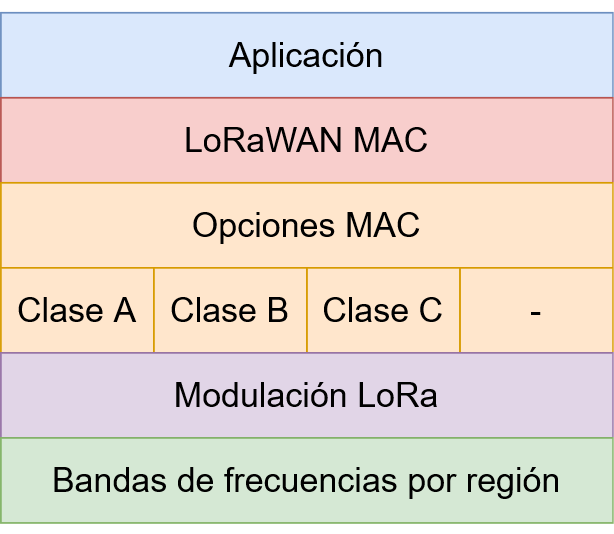
\includegraphics[width=1.0\textwidth]{imagenes/ArquitecturaLoRa.png}
    \caption{Arquitectura LoRa}
    \label{fig:ArquitecturaLoRa}
\end{figure}

\newpage

La topología de red propuesta por LoRaWAN es estrella, es decir, los dispositivos finales se comunican directamente a un salto 
con una estación base de forma bidireccional. Las estaciones base transmiten los datos de los dispositivos finales al servidor de red y viceversa 
utilizando una conexión IP estándar. En la Figura \ref{fig:LoRaWANTopologia} se muestra la arquitectura utilizada en redes LoRa.

\begin{figure}[H]
    \centering
    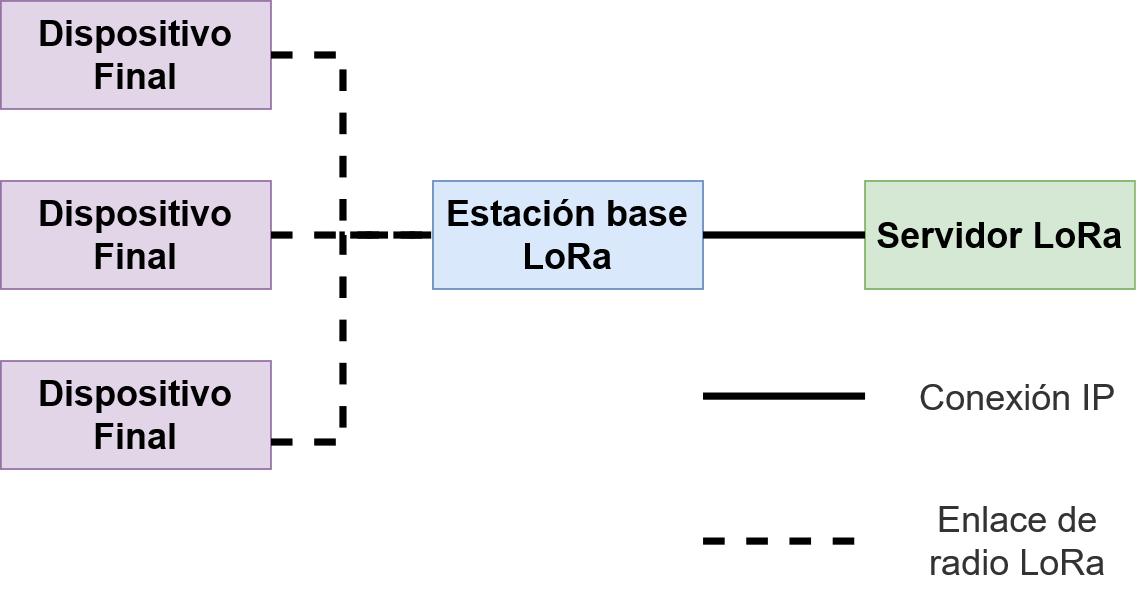
\includegraphics[width=1.0\textwidth]{imagenes/LoRaWANTopologia.png}
    \caption{Topología LoRa}
    \label{fig:LoRaWANTopologia}
\end{figure}

\subsection{Docker}

\gls{Docker} es un motor de contenedores de código libre que utiliza una virtualización\cite{docker_definition} ligera permitiendo automatizar el despliegue de 
aplicaciones mediante \gls{Contenedor} virtuales. Esto significa que puede encapsular las aplicaciones dentro de un contenedor junto con sus dependencias y ejecutarlos sobre 
cualquier equipo que tenga instalada la plataforma \gls{Docker}, usualmente servidores Linux, nubes públicas y privadas. \gls{Docker} amplía LXC con un kernel y una Interfaz de 
Programación de Aplicaciones (API, por sus siglas en inglés) a nivel de aplicación que permiten la ejecución de procesos aislando CPU, memoria, E/S, red, etc. Además, 
Docker utiliza diferentes espacios de nombre para aislar por completo la vista de una aplicación del entorno subyacente (sistema operativo), lo que incluye los árboles de 
procesos, la red, los IDs de usuario y los sistemas de archivos

\subsection{The Things Network}

The Things Network (TTN), es una red de IoT global, descentralizada, gratuita, abierta y en la que cualquier persona puede aportar sus conocimientos acerca de IoT con la finalidad 
de mejorar cada vez más la plataforma. TTN fue creado en el verano de 2015 en Amsterdam, por sus dos fundadores Wienke Giezeman y Johan Stokking\cite{the_things_network_definition}, 
entre otros y cuyo objetivo era facilitar el diseño y la creación de redes, para lo cual daba soporte a las distintas puertas de enlace distribuidos por el mundo y además ofrecía la 
infraestructura de back-end a sus usuarios, es decir, una implementación de las funcionalidades del servidor de red y del servidor de aplicación. 

Este set de herramientas del lado del servidor se enfrenta a duplicidades de mensajes, gestiona la transmisión de mensajes descendentes, gestiona integraciones con plataformas, 
como HTTP o MQTT y ofrece una serie de APIs en diferentes lenguajes de programación como Java, Node.js o Node-Red. 

Como se trata de una plataforma código abierto, los códigos con los que se ha construido el set de herramientas del lado del servidor son públicos y se puede acceder a ellos a 
través de un proyecto en GitHub. Actualmente TTN tiene registradas alrededor de 9000 puertas de enlace distribuidos por todo el mundo y están registrados más de 80000 miembros. 

Teniendo en cuenta que hace tan solo un año había registradas 3000 puertas de enlace, se puede pensar que  la idea de la evolución tan rápida que está teniendo la tecnología 
LoRaWAN y a su vez la red de TTN. En la siguiente Figura \ref{fig:TheThingsStackMap} se puede observar la distribución de las puertas de enlace en el mundo: Este continuo crecimiento de la comunidad permite 
a muchas personas acceder de manera muy sencilla y gratuita a un entorno IoT donde poder realizar proyectos o implementar sus ideas.

\begin{figure}[H]
    \centering
    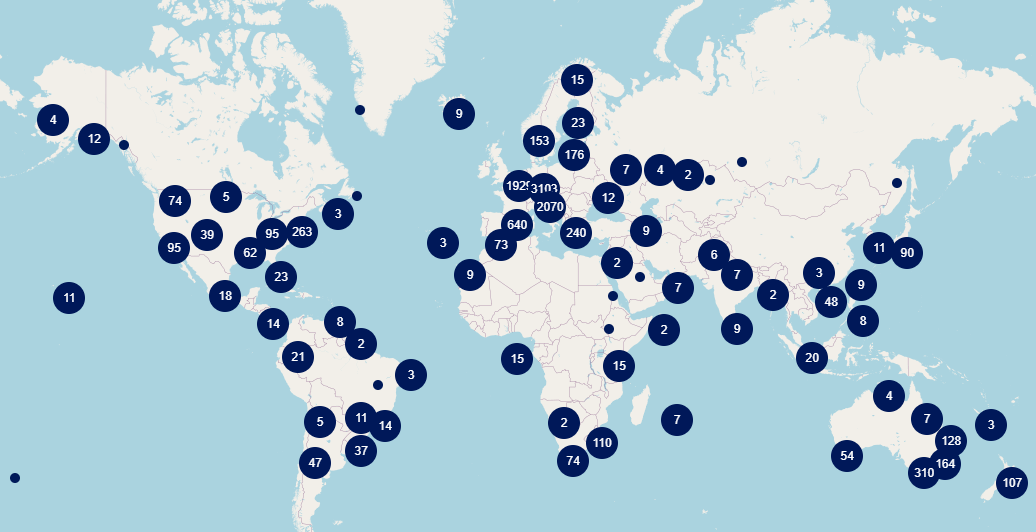
\includegraphics[width=1.0\textwidth]{imagenes/TheThingsStackMap.PNG}
    \caption{Mapa con la distribución de las puertas de enlace en el mundo para The Things Network}
    \label{fig:TheThingsStackMap}
\end{figure}

Además, TTN ha desarrollado una gran cantidad de comunidades en las que los usuarios, generalmente ubicados en las mismas zonas geográficas puedan intercambiar información o 
conocimientos que puedan ser útiles para otros usuarios y así, de manera recíproca pueden servirse de ayuda unos con otros. Por ejemplo, en España se han creado recientemente 
varias comunidades de TTN en Mexico, Estados Unidos, Países en Suramérica, etc., lo cual indica que se está notando el auge de LoRaWAN de forma más cercana.
